\chapter{Gestão de Ativos}
\label{cap-ativos}

\section{Ativos}

\textbf{Definição:} \emph{Dentro da contabilidade, ativo é um recurso econômico. Pode ser considerado qualquer coisa tangível ou intangível. Expressa bens, valores créditos, direitos e assemelhados, que podem gerar valor econômico. Formam o patrimônio de uma pessoa sigular ou coletiva e são avaliados pelo seu custo.} \cite{sullivan2003}\cite{fulgencio2007} 

\textbf{Definição:} \emph{Ativo físico é algo que tem valor real ou potencial para uma organização.
Exemplos: plantas, instalações, equipamentos, estoques, ferramentas, materiais, edifícios, veículos etc.} \cite{nicolay2015}

Ativos são recursos que dão suporte as atividades realizadas por uma organização. E pelas definições acima constata-se que são intrísicos ao seu custo e também geram valor para o negócio. A troca constante desses ativos, por obsolescência, quebra ou falhas, podem gerar custos altos e despesas extras. Por isso é necessário gerí-los de forma adequada, de forma a preservá-los, prolongar seu tempo de vida e ter uma previsão dos gastos necessários para mantê-los. 

Controlar seu ciclo de vida pode ser uma forma de prever falhas, evitá-las e assim melhorar seu desempenho e prolongar seu tempo de uso. A gestão de ativos é uma área que vem sendo valorizada exatamente porque a indústria percebeu a necessidade de diminuir os custos com reparos e substituições.

Marcio Nicolay \cite{nicolay2015} defini vida do ativo e ciclo de vida como:

\textbf{Vida do ativo:} é o período compreendido desde sua criação até o final de sua vida. Sua vida não necessariamente termina depois do descarte.

\textbf{Ciclo de vida:} são todas as etapas envolvidas na gestão de um ativo. Quantidade de etapas e duração variam de acordo com a necessidade da organização.


\section{Normas}

\begin{flushright}
	“\textit{A normalização é tecnologia consolidada, que nos
permite confiar e reproduzir infinitas vezes determinado
procedimento, seja na área industrial, seja no campo de
serviços, ou em programas de gestão, com mínimas
possibilidades de errar...
\\
...
\\
Elaborar uma norma técnica é compartilhar
conhecimento, promover a competitividade, projetar a
excelência e suas melhores consequências nos planos
econômico, social e ambiental.}”
\\
Pedro Buzatto Costa
\\
HISTÓRIA DA NORMALIZAÇÃO BRASILEIRA
\end{flushright}

A citação acima diz em poucas palavras a importância de se ter normas, padrões e especificações que possam assegurar a qualidade em diferentes áreas de conhecimento.

Na área da manutenção e gestão de ativos não é diferente. A preocupação com ativos físicos tem se tornado cada vez mais maior, pois observou-se que garantir a confiabilidade, desempenho, conservar e aumentar o tempo de vida deles pode trazer benefícios significantes, sendo um dos mais importantes, o custo, gastos que podem ser poupados.

\subsection{PAS 55}

Surgiu, em reposta a uma demanda da indútria, o documento PAS 55. Publicada em 2004 pela BSI e revisada em 2008, essa especificação é composta por definições claras e 28 requisitos, considerados necessários para implantar e auditar um eficiente sistema de gestão para todo o ciclo de vida de qualquer ativo físico. A PAS 55 foi dividido em duas parte, traduzidas pela ABRAMAN como:

\begin{itemize}
	\item \textbf{Parte 1:} Especificação para a gestão otimizada de ativos físicos;
	\item \textbf{Parte 2:} Diretrizes para aplicação do PAS 55-1. 
\end{itemize} 

Sua estrutura consiste em um ciclo baseado no PDCA, como mostra a figura abaixo.

\graphicspath{{figuras/}}
\begin{figure}[h]
\centering
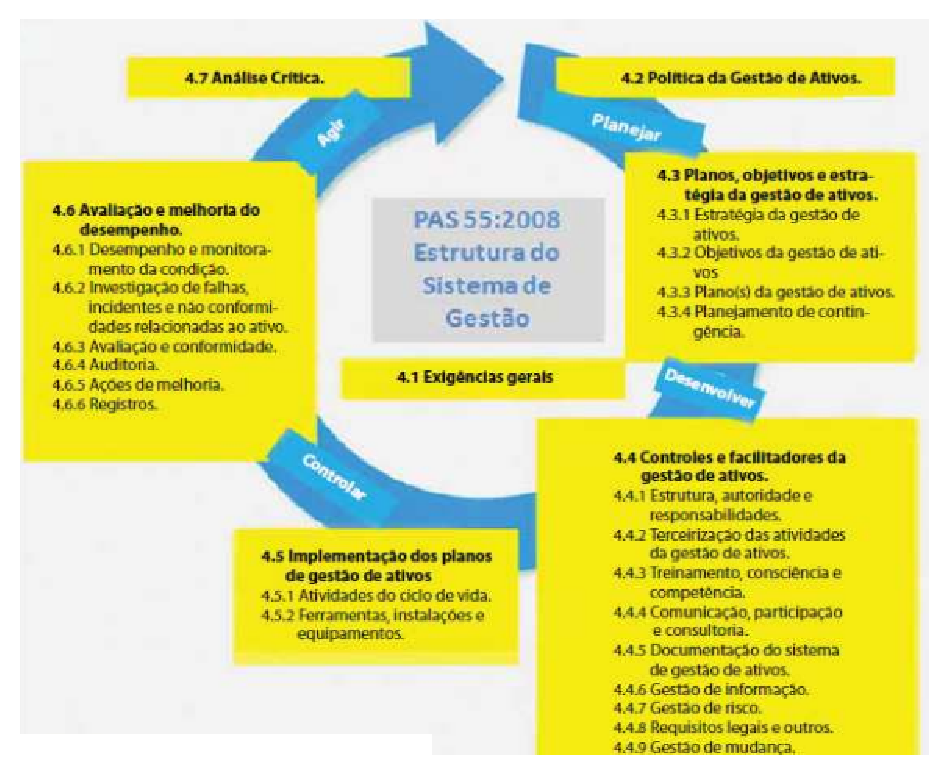
\includegraphics[width=0.8\textwidth]{figura1.eps}
\caption{Estrutura do Sistema de Gestão de Ativos PAS 55. \textbf{Fonte: BSI PAS 55-1:2008.}}
\label{estrututa_pas_55}
\end{figure}

%

A Figura~\ref{estrutura_pas_55} foi adaptada por \cite{valeria2013} e mostra a estrutura do Sistema de Gestão de Ativos. A PAS classifica 5 categorias de ativos:

\begin{enumerate}
	\item{Ativos Físicos}
	\item{Ativos Humanos}
	\item{Ativos de Informação}
	\item{Ativos Financeiros}
	\item{Ativos Intangíveis}
\end{enumerate}

Contudo seu escopo está focado nos \textbf{ativos físicos}. Os outros só são considerados caso estejam realacionados com os ativos.

Segurança, confiabilidade, disponibilidade, infraestrutura e custo são associados a atividades contidas na gestão de ativos. 
Realizar a gestão dos ativos é importante para, conhecer a confiabilidade e a disponibilidade dos sistemas e componentes críticos ao longo do tempo de operação, os riscos inerentes à operação e manutenção, as probabilidades de ocorrências de eventos não desejáveis que afetem a segurança das pessoas e do meio-ambiente.


\subsection{ISO 55000}

A importânia da PAS 55 foi reconhecida quando baseada nela, em janeiro de 2014, foi aprovada a ISO 55000, o primeiro padrão internacional para gestão de ativos. 

A ISO é uma organização internacional e não gonvernamental independente, tendo adesão de 161 organismos necionais de normalização, sendo um deles a ABNT. Seu objetivo é construir padrões internacionais relevantes para o mercado e que deêm suporte a inovação e traga soluções para desafios globais .

